\documentclass[conference]{IEEEtran}
\usepackage{cite}
\usepackage{amsmath,amssymb,amsfonts}
\usepackage{algorithmic}
\usepackage{graphicx}
\usepackage{textcomp}
\usepackage{xcolor}
\usepackage{url}
\usepackage[caption=false]{subfig}

\begin{document}

\title{Numerical Solution and Uncertainty Quantification of Bioheat Transfer Equation Using Neural Network Approach}
\author{\IEEEauthorblockN{Ante Lojić Kapetanović\IEEEauthorrefmark{1},
Anna Šušnjara\IEEEauthorrefmark{2}, Dragan Poljak\IEEEauthorrefmark{3}}
\IEEEauthorblockA{\textit{Faculty of Electrical Engineering, Mechanical Engineering and Naval Architecture}\\
\textit{University of Split}\\
Split, Croatia \\
\IEEEauthorrefmark{1}alojic00@fesb.hr,
\IEEEauthorrefmark{2}asusnja@fesb.hr,
\IEEEauthorrefmark{3}dpoljak@fesb.hr}}

\maketitle

\begin{abstract}
\label{sec.abstract}
The paper deals with a novel approach to carry out uncertainty quantification in modeling of bioheat transfer equation using neural networks and deep learning. The output uncertainty is achieved via Monte Carlo (MC) dropout procedure using Bayesian inference, while the input uncertainty propagation is achieved using MC simulation of the ensemble of physics-informed neural networks (PINNs). The proposed approach uses a neural network with integrated physical knowledge without need of any prior assumptions and mesh generation, respectively. Deterministic modeling is related to both analytical and numerical (finite element method) solution of bioheat transfer equation. The computational example considered in this work pertains to the solution of rather simple one-dimensional problem of bioheat transfer, as a kind of opener to the subject.
\end{abstract}
 
\begin{IEEEkeywords}
bioelectromagnetism, bioheat transfer equation, numerical modeling, physics-informed deep learning, uncertainty quantification
\end{IEEEkeywords}

\section{Introduction}
\label{sec.introduction}
The Pennes’ bioheat transfer equation (PBHTE) is a standard model to tackle the problem of the unknown temperature distribution in the human body tissue \cite{Huang_pbhte_2015}. The thermal input parameters of the PBHTE are not unique, i.e. they differ from one individual to another and, consequently, could be considered as stochastic. Therefore, throughout this study, input parameters of the PBHTE are modeled as random variables of a predetermined statistical distribution thus resulting in related output uncertainty. Important application of the stochastic PBHTE is the hyperthermia therapy (also known as thermal therapy or thermotherapy in literature). It is a malignant disease treatment where patient's body is locally exposed to the appropriate amount of heat generated by an external source \cite{nci_hyperthermia_2011} and is usually an adjunct to chemotherapy and/or radiotherapy. Research has shown that such treatment can kill cancerous cells by damaging proteins and other indispensable structures inside cells \cite{hildebrandt_hyperthermia_2002}, keeping the healthy surrounding tissue intact \cite{vanderzee_hyperthermia_2002}. However, one of the challenges is to expose only local ill area while the rest of the body should not be affected in order to avoid further complications. With the knowledge of the output uncertainty, the decision making process in hyperthermia therapy will be more secure and precise.

This study presents a novel uncertainty quantification approach in modeling PBHTE using neural network modeling and deep learning. The last decade has been marked by the rapid development of numerous branches in deep learning - object recognition in computer vision \cite{krizhevsky_imagenet_2012}, natural language processing and speech recognition, bioinformatics \cite{lecun_dl_2015} and reinforcement learning \cite{silver_go_2016}. Unlike mentioned regimes where the state of the art performance is achieved using deep neural networks and large sets of data, big data acquisition for scientific modeling of physical dynamic processes, such as modeling bioheat transfer in the human body tissue, is computationally expensive. However, there is an ongoing research activity aiming to overcome such problem proposing a novel approach named scientific machine learning \cite{rackauckas2020universal}. The ultimate idea is to integrate knowledge about prior physical domain into a learning algorithm. The information content of the data an algorithm sees is enriched and may quickly converge to the right solution even with a few training examples. The study is further expanded with an uncertainty quantification based on approximate inference using Monte Carlo (MC) dropout, firstly introduced in \cite{gal2015dropout} with the fundamentals carved in research by MacKay, Neal, Barber and Bishop \cite{mackay_bayesian_1992, neal_thesis_1995, mackay_laplace_1998, barber_ensemble_1998}. Additionally, the input uncertainty is propagated through ensemble of neural networks each performing an MC dropout using MC simulation.

The paper is organized as follows: Section \ref{sec.formulation} outlines the formulation of the PBHTE; in Section \ref{sec.analytical-numerical}, the classical approach to PBHTE modeling is described; Section \ref{sec.stochastic-modeling} defines stochastic modeling of previously defined problem, Section \ref{sec.pinn} gives an overview of the neural network based numerical model and stochastic approach; Section \ref{sec.results} is dedicated to the computational results and finally conclusion and discussion together with possible further work are presented in Section \ref{sec.conclusion}.

\section{Formulation}
\label{sec.formulation}
The PBHTE, governing the temperature distribution in the human body tissue, is given with the following expression:
\begin{equation}
\begin{aligned}
\nabla(k \nabla T) + \omega_b \cdot T_a - \omega_b \cdot T + Q_m + Q_{ext} = c_v \rho \frac{\partial T}{\partial t}
\end{aligned}
\label{eqn.bioheat}
\end{equation}
where $\rho$, $c$, $k$ are respectively the density, the specific heat, and the thermal conductivity of the tissue; $\rho_b$ and $c_b$ denote density and specific blood heat; $\omega_b$ is the blood perfusion; $T_a$ is the arterial temperature, and $T$ stands for the tissue temperature. $Q_m$ is the metabolic heat generation, and $Q_{ext}$ is the heat source due to spatial heating \cite{deng_bioheat_2002}.

For the sake of simplicity, instead of the general form PBHTE given in \eqref{eqn.bioheat}, the steady state will be considered. Therefore, the time-invariant PBHTE can be written as:
\begin{equation}
\begin{aligned}
\nabla(k \nabla T) + \omega_b \cdot T_a - \omega_b \cdot T + Q_m + Q_{ext} = 0
\end{aligned}
\label{eqn.bioheat-time-inv}
\end{equation}

Finally, as an opener to the subject, a rather simple one-dimensional case is analyzed. Hence, a solution domain of interest $\Omega$ is defined as the one-dimensional space $x \in [0, L]$, $x \subseteq \Omega$, $\Omega \subset \mathbb R^1$, and $L$ is the tissue depth, here considered to be 3 cm. The geometry of the problem is depicted in Fig. \ref{fig.geometry}. Note that the heat is generated perpendicular to the skin and there is no influence of the external heat source at tissue depth $L$.
\begin{figure}[]
\centering
 \includegraphics[width=\linewidth]{figs/geometry(1).pdf}
\caption{The geometry of the problem - heat generation onto the localized body area.}
\label{fig.geometry}
\end{figure}
The corresponding one-dimensional equivalent of \eqref{eqn.bioheat-time-inv}, with no external heat generated to the skin, is given by:
\begin{equation}
\begin{aligned}
k \frac{d^2 T(x)}{dx^2} + \omega_b \cdot T_a - \omega_b \cdot T(x) + Q_m = 0
\end{aligned}
\label{eqn.bioheat-1d-time-inv}
\end{equation}
with Robin and Dirichlet boundary conditions:
\begin{equation}
    \begin{cases} 
    -k \frac{dT_0(x)}{dx} = h_0[T_f - T_0(x)],& \mbox{for } x=0 \\ 
    T_L(x) = T_c,& \mbox{for } x=L
    \end{cases}
\label{eqn.bcs}
\end{equation}
where $h_0$, $T_c$ and $T_f$ are the convection coefficient, the body core temperature and the atmospheric temperature, respectively. 

The input thermal parameters $k$, $\omega_b$, $T_a$, $Q_m$, $h_0$ and $T_f$ are treated as uniformly distributed random variables with 20\% variation coefficient \cite{anna_bioheat_2019}. The nominal values of all input parameters are given in Table \ref{table.params}.
\begin{table}[htbp]
\caption{The expected values for the thermal input parameters}
\begin{center}
\begin{tabular}{|c|c|}
\hline
\textbf{Parameter} & \textbf{Expected value}\\
\hline
$\rho$, $\rho_b$ & 1000 $kg/m^3$\\
\hline
$c$, $c_b$ & 4200 $J/kg {}^\circ C$\\
\hline
$T_a$, $T_c$ & ${37}^\circ C$\\
\hline
$T_f$ & ${25}^\circ C$\\
\hline
$k$ & 0.5 $W/m {}^\circ C$\\
\hline
$\omega_b$ & 2100 $kg/sm^3$\\
\hline
$Q_m$ & 33800 $W/m^3$\\
\hline
$h_0$ & 10 $W/m^2 {}^\circ C$\\
\hline
$h_f$ & 100 $W/m^2 {}^\circ C$\\
\hline
\end{tabular}
\label{table.params}
\end{center}
\end{table}
Within the framework of the deterministic modeling the one dimensional problem formulated by \eqref{eqn.bioheat-1d-time-inv} and \eqref{eqn.bcs} can be solved via analytical and numerical procedure, respectively. The details to follow are given in Section \ref{sec.analytical-numerical}.


\section{Analytical and Numerical Solution}
\label{sec.analytical-numerical}
The accuracy of the deterministic model and the novel neural network optimization method is verified by the corresponding analytical solution. For the sake of completeness, the analytical solution is given in Appendix \ref{ap.an}, while the mathematical details could be found elsewhere, e.g. in \cite{deng_bioheat_2002}.
Furthermore, the numerical solution of \eqref{eqn.bioheat-1d-time-inv} via Finite Element Method (FEM) is outlined in Appendix \ref{ap.fem}. Again, the full mathematical description is available in number of references, e.g. in \cite{poljak_bioem_2018}.

It is well-known fact that FEM, as very powerful numerical tool, requires a generation of mesh (which appears to be pretty demanding for realistic highly irregular and non-homogeneous computational domains), a fine grained solution domain approximation where linear combination of polynomials is used to express a local solution over a finite element whose accuracy appreciably depends on the resolution of the mesh for a particular problem of interest.
The temperature distribution obtained both analytically and via 20 finite elements using linear interpolation over an element is shown Fig. \ref{fig.fem}. Here, the nominal values of input parameters from Table \ref{table.params} are used.
\begin{figure}[]
\centering
 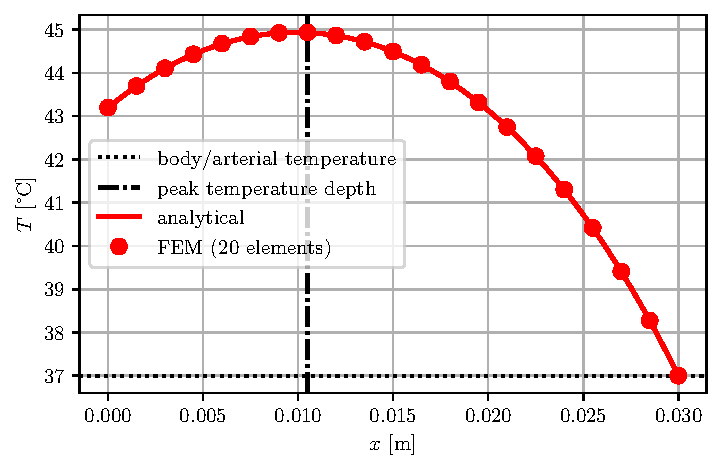
\includegraphics[width=\linewidth]{figs/FEM-20felems.pdf}
\caption{FEM solution using linear test and base functions.}
\label{fig.fem}
\end{figure}

\section{Stochastic Modeling via Monte Carlo Method}
\label{sec.stochastic-modeling}
The PBHTE output uncertainty is quantified by implementing the MC sampling method, widely shown to be robust and accurate approach in uncertainty quantification.
Generally, the MC sampling method is purely statistical method that relies on repeated random sampling of input parameters, based on some predefined probability distribution. 
For each sample, the input parameters are fixed and the problem becomes deterministic. The ensemble of solutions is obtained by iteratively applying a numerical method to each sample of randomly generated input parameters. From here, the statistics such as mean and variance can be extracted.
The biggest disadvantage of the MC sampling method lies in its iterative nature where, in order to acquire high accuracy on the output, a large number of samples is required \cite{xiu_stochasticism_2009}.

In this paper, 100 realizations with 100 samples each has been used within the framework of the Monte Carlo method and for each method the results have been obtained by using analytical solution, for details see Appendix \ref{ap.an} The total final uncertainty quantification of the ensemble of results is depicted in Fig. \ref{fig.mc}.
\begin{figure}[]
\centering
 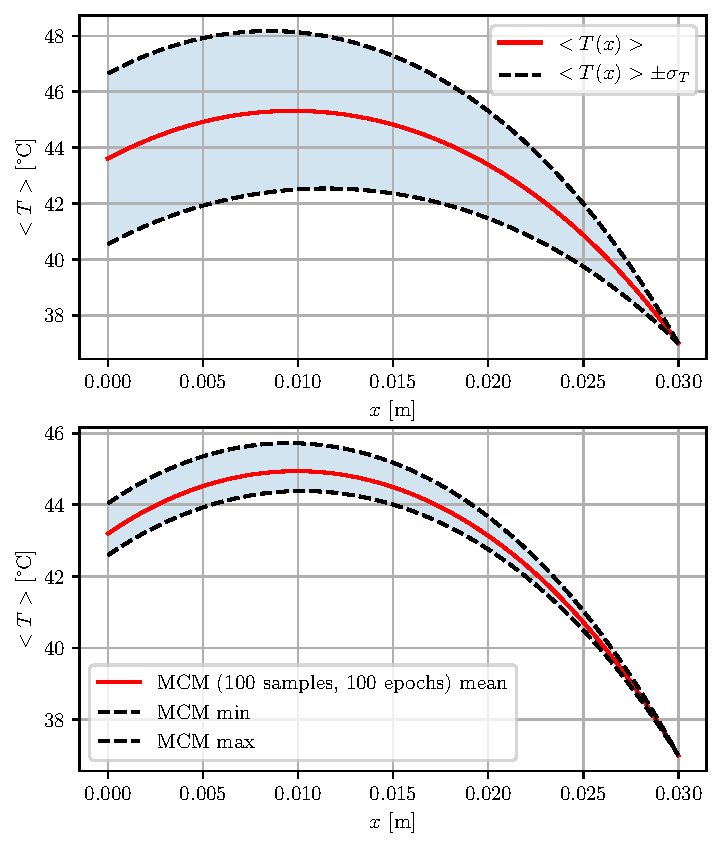
\includegraphics[width=\linewidth]{figs/mc-simulation-100epochs-100samples.pdf}
\caption{The upper plot depicts single sample expectation inside 95\% confidence interval and lower plot depicts Monte Carlo simulation with 100 iterations.}
\label{fig.mc}
\end{figure}
It can be observed that the results obtained via MC sampling method are normally distributed, even though, in this case, samples have been obtained from uniformly distributed input thermal parameters. This phenomenon, shown in Fig. \ref{fig.mc-distribution}, is well-known in statistical analysis and stems from the \emph{central limit theorem}.
\begin{figure}[]
\centering
 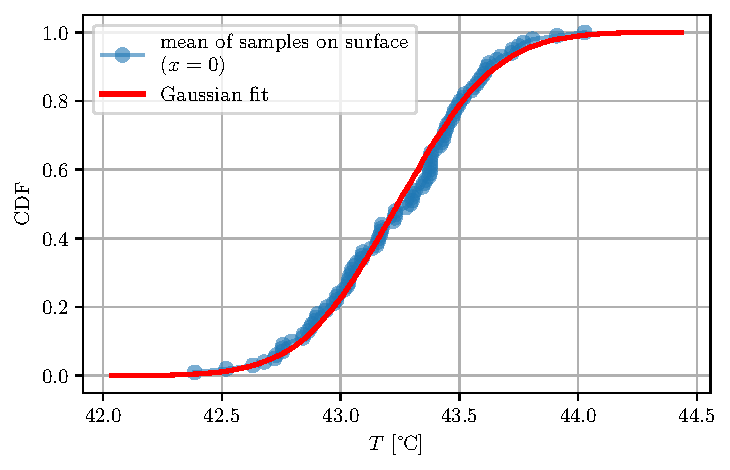
\includegraphics[width=\linewidth]{figs/mc-distribution.pdf}
\caption{The visual proof of central limit theorem: expected values of each sample for the $x=0$ are shown as cumulative distributed function and are compared with Gaussian distribution.}
\label{fig.mc-distribution}
\end{figure}

\section{Numerical Solution and Stochastic Modeling using Physics-Informed Neural Networks}
\label{sec.pinn}
The most of the engineering and physics dynamical real-world problems are described through non-linear partial differential equations (PDEs). Even though neural network based numerical solvers for ordinary differential equations (ODEs), a system of ODEs and PDEs were developed in late 1990s by Lagaris et al. \cite{lagaris_ann_1998}, assuming that neural networks in fact are universal function approximators \cite{hornik_ufa_1989}, only recently physics-informed neural networks (PINNs), introduced by Raissi et al. in \cite{raissi_pinn_2018}, have reached full capacity by exploiting advances of the automatic differentiation. % \cite{tensorflow2015-whitepaper}.

In this study, DeepXDE Python library \cite{lu_deepxde_2019} was used because of its high-level abstraction syntax, which closely resembles the mathematical formulation without losing the usability and customizability. The first step is to represent the solution $T(x)$ with a neural network $\hat{T}(x)$ where $x$ is the spatial coordinate of the PBHTE and the input data for the PINN. This PINN is a fully connected multi-layer perceptron (MLP), which applies linear and nonlinear transformations to the inputs recursively. It is consisted of a single unit input layer, three hidden layers with fifty units each, and a single unit output layer. Each unit activates its input using hyperbolic tangent activation function. Regularization is applied through the embedded underlying physical knowledge and by adding dropout after each layer. The latter regularization procedure enables quantification of the output uncertainty, which is discussed subsequently in the section. The full neural network $\hat T(x;\theta)$ architecture, where $\theta$ is the vector of neural network parameters, along with the restriction of the neural network to satisfy the physics that comes from underlying dynamics of the PBHTE and known boundary conditions is shown in Fig. \ref{fig.bioheatnn}.
\begin{figure*}[ht]
  \centering
  \includegraphics[width=\textwidth]{figs/bioheatnn.pdf}
  \caption{PINN configuration for solving the PBHTE with mixed boundary conditions, where the multi-layer perceptron is function $T(x)$ approximator, after which PDE and boundary conditions are defined and finally loss function $J(\theta)$ is constructed.}
  \label{fig.bioheatnn}
\end{figure*}

PINNs, at their core, are mesh-free PDE solvers and are learned by a gradient-based optimizer, where the end goal is the minimization of the loss function. The loss function can be written as the weighted summation of the $l^2$ norm of residual points for the solution domain $\tau_d$ and for the boundary $\tau_b$:
\begin{equation}
\begin{aligned}
    J(\theta; \tau) = & w_d \cdot \frac{1}{\tau_d} \sum_{x \in \tau_f} \lVert k \cdot \frac{\partial^2 \hat{T}}{\partial x^2} - w_b \cdot \hat{T} + w_b \cdot T_a + Q_m \lVert^2 \\
    & + w_b \cdot \frac{1}{\tau_b} \sum_{x \in \tau_b} \Big( \lVert -k \cdot \frac{d \hat{T}}{dx} + h_0 \cdot (\hat{T}|_{x=0} - T_f) \lVert^2\\
    &\quad\quad\quad\quad\quad\quad+ \lVert \hat{T}|_{x=L} - T_c \lVert^2 \Big)
\end{aligned}
\label{eqn.loss}
\end{equation}
where $w_d$ and $w_b$ are weights initialized using Xavier initialization scheme \cite{glorot_bengio_2010}. 
$\tau_d$ represents the set of randomly scattered data points in the solution domain $\Omega$, captured as the training data.
Having constructed the loss function, training is performed using Adam, the first-order stochastic gradient-based optimization algorithm, introduced in \cite{kingma_adam_2014}. 

Since the problem of solving the PBHTE is transformed to the optimization problem, solutions will slightly differ for each run. Absolute precision is not possible due to the non-convex nature of the loss function, but high precision is possible using fine tuned hyperparameters such as the learning rate, the number of residual points, loss weights and the number of layers and units per layer.

Uncertainty quantification of the output is achieved using dropout method which "drops" units from the network randomly with some probability $p$. Dropout procedure is performed for the regularization purposes and is carried out during the training period. By using dropout during test time, the stochastic prediction on the output is achieved, where the mean of the output is directly estimated by the MC method:
\begin{equation}
    \mathop{\mathbb{E}}(T|x; \theta) \approx \frac{1}{N_{test}}\sum_{n=1}^{N_{test}} \hat{T}(x)
    \label{eqn.mcdropout}
\end{equation}
where $N_{test}$ is the total number of test samples.

\section{Results and Discussion}
\label{sec.results}
The number of training points was chosen in order to match the number of finite elements for FEM, Section \ref{sec.analytical-numerical} of the paper.
The neural network was trained on 20 training points in the solution domain $x \in [0, L]$ where $x \subseteq \Omega$ and $\Omega \in \mathbb R ^1$ with integrated underlying physical knowledge for 10,000 epochs. The obtained results are shown in Fig. \ref{fig.regression}. The regression at the defined interval across 100 test points is shown in Fig. \ref{fig.regression-mean}, while Fig. \ref{fig.regerssion-uncertainty} shows the expectation of the neural network output located within the 95\% confidence interval (CI). The regression line is in excellent agreement with true values obtained analytically. 
\begin{figure}[!t]
\centering
\subfloat[]{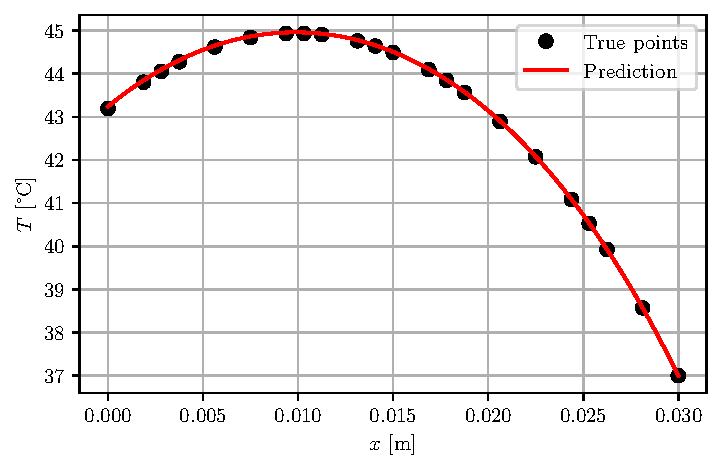
\includegraphics[clip,width=\columnwidth]{figs/regression-mean.pdf}
\label{fig.regression-mean}}
\hfil
\subfloat[]{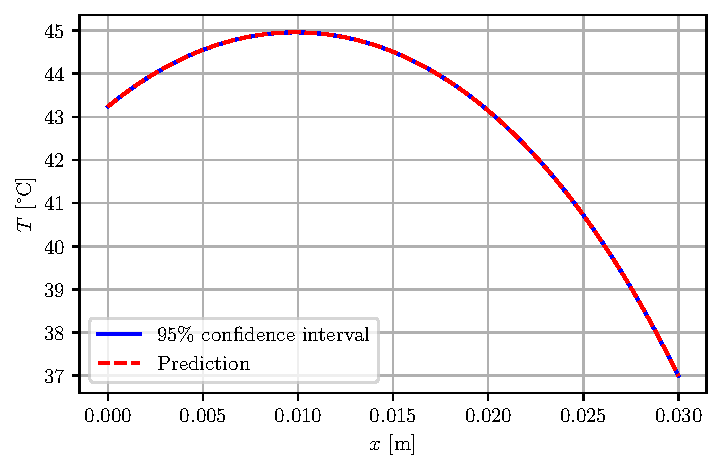
\includegraphics[clip,width=\columnwidth]{figs/regression-uncertainty.pdf}
\label{fig.regerssion-uncertainty}}
\caption{The neural network output within 95\% CI after ten thousands training iterations. The hyperparameter search is performed manually, where the best results are obtained using the learning rate of 0.001 and $l_2$ relative error as loss metrics. Adam optimization was used in order to minimize the loss function \eqref{eqn.loss} and obtain optimal $\theta_{opt}$.}
\label{fig.regression}
\end{figure}
The learning curves, depicted in Fig. \ref{fig.loss}, show that a small number of training points is sufficient to achieve low values of the loss function on test set.
\begin{figure}[!t]
\centering
 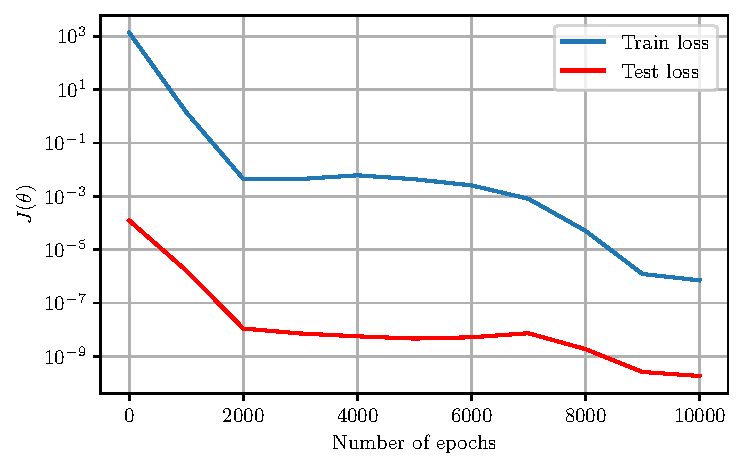
\includegraphics[width=\linewidth]{figs/loss.pdf}
\caption{Learning curves show the values of the loss function during training and testing with respect to number of training epochs.}
\label{fig.loss}
\end{figure}

MC dropout, when applied during the testing time provides uncertainty quantification of the output, is not satisfactory method for uncertainty analysis when the input thermal parameters of the PBHTE are treated as random variables, as stated in Section \ref{sec.formulation}. In order to tackle this problem, the neural network ensemble is trained using a sort of Monte Carlo method where input parameters are considered uniformly distributed with respect to a nominal mean value and 20\% variation coefficient, and are sampled 5 times with 5 different expectation values in each sampling. Overall, 25 neural networks were trained on the sampled data and the final output is shown in Fig. \ref{fig.ensamble}.
\begin{figure}[]
\centering
 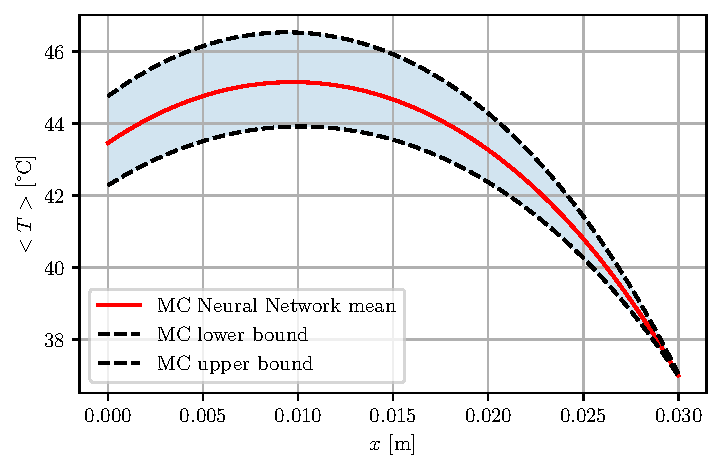
\includegraphics[width=\linewidth]{figs/uncertainty-mcnn-5epochs5samples.pdf}
\caption{Monte Carlo method using the same feed forward neural network. For 5 random variables taken as uncertain input, we run the simulation for 5 times. Resulting graph shows expected value using red regression line inside the confidence interval constructed as area between the outputs with the lowest and highest value during the simulation.}
\label{fig.ensamble}
\end{figure}

\section{Conclusion}
\label{sec.conclusion}
This paper deals with a novel approach to uncertainty quantification in modeling of PBHTE using neural networks and deep learning. The work aims to demonstrate the ability of the neural network as the universal function approximator to successfully converge to the correct solution on the given solution domain, with extremely low error measured on a test set. The R2 score is 99.9863\% measured on 100 test points. Uncertainty of the output is achieved using MC dropout procedure. This method uses Bayesian inference where the probability distribution of the output is based on the prior distribution of hyperparameters and the likelihood of the output. The input uncertainty propagation is achieved using the ensemble of PINNs trained on uniformly distributed input parameters using MC method.

The main advantage of the approach proposed in this paper over the classic numerical methods is the construction of a neural network with integrated physical knowledge without any prior assumptions and without the need of mesh generation, respectively. Moreover, instead of transforming the PBHTE to an algebraic system, PINNs engrave both the equation and boundary conditions into the loss function, thus transforming the problem of modeling the heat transfer in biological tissues to the optimization problem. The method does not depend neither on the complexity of the computational domain geometry nor on the dimensionality of the problem. 
%OSIM IREGULARNOSTI GEOMETRIJE U DOZIMETRIJI NAILAZIMO NA PROBLEM NEHOMOGENOSTI. komentar
The future work will directly address the problems of solving multidimensional problems of complex geometries in the field of (bio)electromagnetism.

\section*{Acknowledgment}
This research has been funded by DATACROSS project of The Centre of Research Excellence for Data Science and Advanced Cooperative Systems (CRE ACROSS-DataScience).

\appendices
\renewcommand{\theequation}{\thesection.\arabic{equation}}
\setcounter{equation}{0}
\section{Analytical Solution of the PBHTE}
\label{ap.an}
Analytical solution of the BPHTE, defined by \eqref{eqn.bioheat-1d-time-inv}, with mixed boundary conditions, Robin's for $x=0$ and Dirichlet's for $x=L$, is given in \cite{deng_bioheat_2002}. This solution represents the temperature distribution for the steady state of the human body tissue and it is written in the following equation:
\begin{equation}
\begin{aligned}
    T_0(x) & =  T_a + \frac{Q_m}{\omega_b \rho_b c_b} \\
     &+ \frac{\Big(T_c - T_a - \frac{Q_m}{\omega_b \rho_b c_b} \Big) \Big[\sqrt{A}ch(\sqrt{A}x) + \frac{h_0}{k}sh(\sqrt{A}x) \Big]}{\sqrt{A}ch(\sqrt{A}L) + \frac{h_0}{k}sh(\sqrt{A}L)}\\
     &+\frac{\frac{h_0}{k}\big(T_f - T_a - \frac{Q_m}{\omega_b \rho_b c_b} \big)\cdot sh\big[\sqrt{A}(L-x)\big]}{\sqrt{A}ch(\sqrt{A}L) + \frac{h_0}{k}sh(\sqrt{A}L)}
    \label{eqn.analytical_sol}
\end{aligned}
\end{equation}
with
\begin{equation}
\begin{aligned}
    A = \frac{\omega_b \rho_b c_b}{k}
    \label{eqn.a}
\end{aligned}
\end{equation}

\renewcommand{\theequation}{\thesection.\arabic{equation}}
\setcounter{equation}{0}
\section{Solution of the PBHTE via Finite Element Method }
\label{ap.fem}
According to the standard FEM algorithm, featuring weighted residual approach, the PBHTE \eqref{eqn.bioheat-1d-time-inv} is multiplied by the set of weight functions $w_j$ and the following expression is obtained
\begin{equation}
\begin{aligned}
    \int_{0}^{L}\Big[ k \cdot \frac{\partial^2 T}{\partial x^2} - \omega_b \cdot T + \omega_b \cdot T_a + Q_m \Big ] w_j(x) dx = 0    \label{eqn.weighted-residual-method}
\end{aligned}
\end{equation}
where, $w_j$ are weight functions for $j=0,1,2,...$.

Temperature values over the solution domain can then be approximated as a polynomial expansion over a set of basis functions:
\begin{equation}
\begin{aligned}
    \hat{T}(x) = \sum_i \hat{T}_i \cdot N_i(x)
    \label{eqn.fem-approximation}
\end{aligned}
\end{equation}
$N_i$ are basis functions for $i=0,1,2,..$.

Inserting \eqref{eqn.fem-approximation} into weighted residual integral \eqref{eqn.weighted-residual-method}, utilizing the weak formulation of the problem and applying the FEM dsicretization with Galerkin-Bubnov procedure, the following expression is obtained:
\begin{equation}
\begin{aligned}
    \sum_i^{M}  \hat{T}_i\left\Bigg\{ &k \cdot N_j(x) \cdot \frac{\partial N_i(x)}{\partial x}|_{boundary} \\
    & - \int_{x_i}^{x_i + \Delta x}k \cdot \frac{\partial N_i(x)}{\partial x} \cdot \frac{\partial N_j(x)}{\partial x}dx \\
    & - \int_{x_i}^{x_i + \Delta x}\omega_b \cdot N_i(x) \cdot N_j(x)dx \\
    & + \int_{x_i}^{x_i + \Delta x}\big( \omega_b \cdot T_a + Q_m \big)N_j(x) dx \right\Bigg\} = 0   
\end{aligned}
\label{eqn.weak-form}
\end{equation}
for $i=1,2,...,M$, and  $j=1,2,...,M$ where $M$ stands for total number of elements. $N_i$ denotes the linear shape functions, while $x_i$ and $x_i + \Delta x$ are local points of $i$-th element and $\Delta x= \frac{L}{M}$ is the length of an 1-D element.

From \eqref{eqn.weak-form}, global matrix system is assembled, which can be, for convenience, written, as follows
\begin{equation}
\mbox{\textbf{LHS}} \times \mbox{\textbf{T}}= \mbox{\textbf{RHS}}
\label{eqn.assemble}
\end{equation}
where $\mbox{\textbf{LHS}}$ is
\begin{equation}
\begin{aligned}
   \mbox{\textbf{LHS}}_{ji}^k = &\int_{x_i}^{x_i + \Delta x}k \cdot \frac{\partial N_i(x)}{\partial x} \cdot \frac{\partial N_j(x)}{\partial x}dx \\
   &- \int_{x_i}^{x_i + \Delta x}\omega_b \cdot N_i(x) \cdot N_j(x)dx  
\end{aligned}
\label{eqn.lhs}
\end{equation}
and $\mbox{\textbf{RHS}}$ is given by
\begin{equation}
\begin{aligned}
   \mbox{\textbf{RHS}}_{j}^k = & - \int_{x_i}^{x_i + \Delta x}\big(\omega_b \cdot T_a + Q_m\big) \cdot  N_j(x)dx
\end{aligned}
\label{eqn.rhs}
\end{equation}
The vector of values for temperature distribution is obtained by solving the matrix system \eqref{eqn.assemble} after incorporating the prescribed boundary conditions.

\bibliographystyle{IEEEtran}
\bibliography{./bibl}

\end{document}

% helpers
%%%%%%%%%%%
% adding figures in single column
%%%%%%%%%%%%%%%%%%%%%%%%%%%%%%%%%
%\begin{figure}[]
%\centering
% 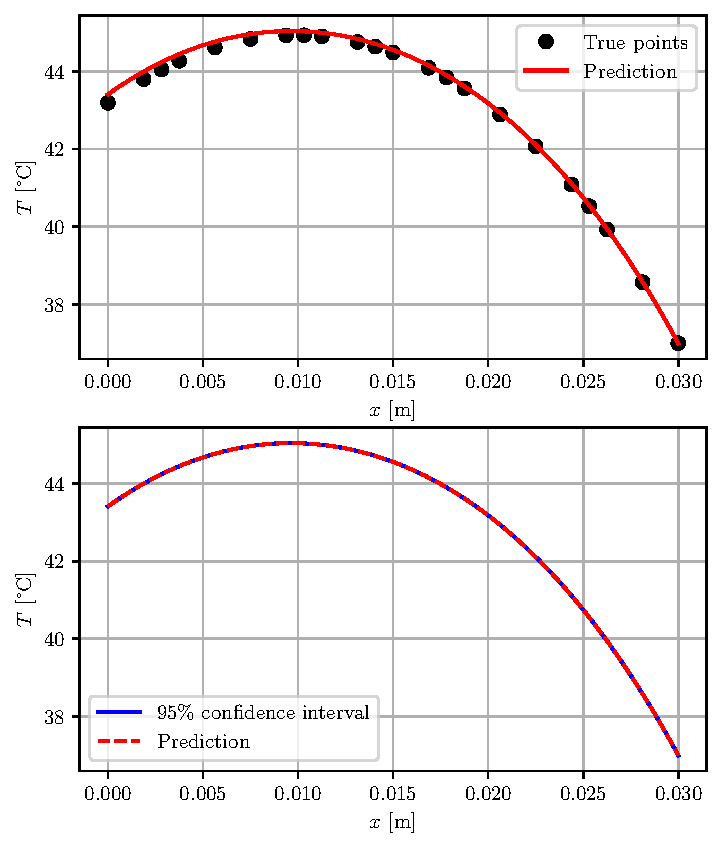
\includegraphics[width=\linewidth]{figs/regression.pdf}
%\caption{Neural network's output}
%\label{fig.regression}
%\end{figure}

% adding figures over two columns
%%%%%%%%%%%%%%%%%%%%%%%%%%%%%%%%%
%\begin{figure*}[h]
%  \includegraphics[width=\textwidth]{figs/bioheatnn.pdf}
%  \caption{NN}
%\end{figure*}

